% documentclass options:
% ngerman is needed for hyphenation if the thesis contains parts written in German
% BCOR is binding correction
% if you'd rather have a one sided thesis, add `oneside' to the documentclass
\documentclass[11pt,
  a4paper,
  % parskip=half, % This is some extra vertical space between paragraphs, the suggestion is 2cm which is really ugly, so we use what koma script gives us
  % you can also set it to full for even more space. But there is a bad tex style decision: parskip also changes the spacing between listitems such as
  % enumerate and itemize. For this purpose we include the enumitem package and set itemsep=.5em, of course you can change this
  BCOR=10mm,
  english,
  ngerman]{book}
\usepackage[english, ngerman]{babel} % If you write mainly in english change order to ngerman, english
% Include of titling must happen before \title etc.
% that's why it's not in setup.tex
\usepackage{titling}
\title{Your title goes here}
\author{Your Name}

% include all packages and define commands in setup.tex

%------------------------------------------------------------------------------
%       package includes
%------------------------------------------------------------------------------
    % font encoding is set up for pdflatex, for other environments see
    % http://tex.stackexchange.com/questions/44694/fontenc-vs-inputenc
    \usepackage[T1]{fontenc}  % 8-bit fonts, improves handling of hyphenations
    \usepackage[utf8x]{inputenc}
    % provides `old' commands for table of contents. Eases the ability to switch
    % between book and scrbook
    \usepackage{scrhack}


    % ------------------- layout, default -------------------
    % adjust the style of float's captions, separated from text to improve readabilty
    \usepackage[labelfont=bf, labelsep=colon, format=hang, textfont=singlespacing]{caption}
    \usepackage{chngcntr}  % continuous numbering of figures/tables over chapters
    \counterwithout{equation}{chapter}
    \counterwithout{figure}{chapter}
    \counterwithout{table}{chapter}

    % Uncomment the following line if you switch from scrbook to book
    % and comment the setkomafont line
    %\usepackage{titlesec}  % remove "Chapter" from the chapter title
    %\titleformat{\chapter}[hang]{\bfseries\huge}{\thechapter}{2pc}{\huge}
    \setkomafont{chapter}{\normalfont\bfseries\huge}

    \usepackage{setspace}  % Line spacing
    \onehalfspacing 
    % \doublespacing  % uncomment for double spacing, e.g. for annotations in correction

    % ------------------- functional, default-------------------
    \usepackage[dvipsnames]{xcolor}  % more colors
    \usepackage{array}  % custom format per column in table - needed on the title page
    \usepackage{graphicx}  % include graphics
    \usepackage{subfig}  % divide figure, e.g. 1(a), 1(b)...
    \usepackage{amsmath}  % |
    \usepackage{amsthm}   % | math, bmatrix etc
    \usepackage{amsfonts} % |
    \usepackage{calc}  % calculate within LaTeX
    \usepackage[unicode=true,bookmarks=true,bookmarksnumbered=true,
                bookmarksopen=true,bookmarksopenlevel=1,breaklinks=false,
                pdfborder={0 0 0},backref=false,colorlinks=false]{hyperref}


    %==========================================
    % You might not need the following packages, I only included them as they
    % are needed for the example floats
    % ------------------- functional, custom -------------------
    \usepackage{algorithm,algpseudocode}
    \usepackage{bm}  % bold greek variables (boldmath)
    \usepackage{tikz}
    \usetikzlibrary{positioning}  % use: above left of, etc


%------------------------------------------------------------------------------
%       (re)new commands / settings
%------------------------------------------------------------------------------
    % ----------------- referencing ----------------
    \newcommand{\secref}[1]{Section~\ref{#1}}
    \newcommand{\chapref}[1]{Chapter~\ref{#1}}
    \renewcommand{\eqref}[1]{Equation~(\ref{#1})}
    \newcommand{\figref}[1]{Figure~\ref{#1}}
    \newcommand{\tabref}[1]{Table~\ref{#1}}

    % ------------------- colors -------------------
    \definecolor{darkgreen}{rgb}{0.0, 0.5, 0.0}
    % Colors of the Albert Ludwigs University as in
    % https://www.zuv.uni-freiburg.de/service/cd/cd-manual/farbwelt 
    \definecolor{UniBlue}{RGB}{0, 74, 153}
    \definecolor{UniRed}{RGB}{193, 0, 42}
    \definecolor{UniGrey}{RGB}{154, 155, 156}


    % ------------------- layout -------------------
    % prevents floating objects from being placed ahead of their section
    \let\mySection\section\renewcommand{\section}{\suppressfloats[t]\mySection}
    \let\mySubSection\subsection\renewcommand{\subsection}{\suppressfloats[t]\mySubSection}


    % ------------------- marker commands -------------------
    % ToDo command
    \newcommand{\todo}[1]{\textbf{\textcolor{red}{(TODO: #1)}}}
    \newcommand{\extend}[1]{\textbf{\textcolor{darkgreen}{(EXTEND: #1)}}}
    % Lighter color to note down quick drafts
    \newcommand{\draft}[1]{\textbf{\textcolor{NavyBlue}{(DRAFT: #1)}}}


    % ------------------- math formatting commands -------------------
    % define vectors to be bold instead of using an arrow
    \renewcommand{\vec}[1]{\mathbf{#1}}
    \newcommand{\mat}[1]{\mathbf{#1}}
    % tag equation with name
    \newcommand{\eqname}[1]{\tag*{#1}}


    % ------------------- pdf settings -------------------
    % ADAPT THIS
    \hypersetup{pdftitle={The great title!},
                pdfauthor={FirstName LastName},
                pdfsubject={Undergraduate thesis at the Albert Ludwig University of Freiburg},
                pdfkeywords={deep learning, awesome algorithm,  undergraduate thesis},
                pdfpagelayout=OneColumn, pdfnewwindow=true, pdfstartview=XYZ, plainpages=false}


    %==========================================
    % You might not need the following commands, I only included them as they
    % are needed for the example floats

    % ------------------- Tikz styles -------------------
    \tikzset{>=latex}  % arrow style


    % ------------------- algorithm ---------------------
    % Command to align comments in algorithm
    \newcommand{\alignedComment}[1]{\Comment{\parbox[t]{.35\linewidth}{#1}}}
    % define a foreach command in algorithms
    \algnewcommand\algorithmicforeach{\textbf{foreach}}
    \algdef{S}[FOR]{ForEach}[1]{\algorithmicforeach\ #1\ \algorithmicdo}


\begin{document}
    \pagestyle{empty} % no header and no page number
    % disable hyper links to remove warning "destination with same identifier"
    % this means within this section nothing can be referenced with a hyperlink
    \hypersetup{pageanchor=false}

    % enable/disable, depending on your chosen language
    
\begin{titlepage}
\begin{center}

\newcommand{\HorizontalLine}{\rule{\linewidth}{0.3mm}}

{\Large Undergraduate/Master's Thesis}\\[1.3cm]


% _____________________________________________________________________________
\HorizontalLine \\[0.4cm]
% Write your title in a fancy way like this if you want to customize it, otherwise simply let tex do it for you
% \begin{spacing}{3}
%     {\huge \bfseries The Long, Long } \\
%     {\huge \bfseries Long Long} \\
%     {\huge \bfseries Title}\\
% \end{spacing}
{ \huge \bfseries \thetitle }
\HorizontalLine \\[1.5cm]
% _____________________________________________________________________________


{\Huge \theauthor} \\[2cm]


\begin{tabular}[hc]{>{\huge}l >{\huge}l}
  Examiner: & Prof. Dr. Bugs Bunny \\[0.3cm]
  Advisers: & Terence Hill, Bud Spencer \\[1.2cm]
\end{tabular}
\vfill  % move the following text to the bottom

\Large {
    Albert-Ludwigs-University Freiburg\\
    Faculty of Engineering\\
    Department of Computer Science\\
    Chair for Thesis Templates\\[1cm]

    October 05\textsuperscript{th}, 2016\\
}
\end{center}
\end{titlepage}

\thispagestyle{empty}
% title page back
\ \vfill \ \\  % at least one space required before vfill
\
\textbf{Writing period}            \smallskip{} \\
05.\,07.\,2016 -- 05.\,10.\,2016   \bigskip{} \\
\
\textbf{Examiner}                  \smallskip{} \\
Prof. Dr. Bugs Bunny               \bigskip{} \\
\
\textbf{Advisers}                  \smallskip{} \\
Terence Hill, Bud Spencer

    
\begin{titlepage}
\begin{center}

\newcommand{\HorizontalLine}{\rule{\linewidth}{0.3mm}}

{\Large Bachelor/Master Thesis}\\[1.3cm]


% _____________________________________________________________________________
\HorizontalLine \\[0.4cm]
\begin{spacing}{3}
    {\huge \bfseries Der Lange, Lange } \\
    {\huge \bfseries Lange Lange} \\
    {\huge \bfseries Titel}\\
\end{spacing}
\HorizontalLine \\[1.5cm]
% _____________________________________________________________________________


{\Huge Dein Name} \\[2cm]


\begin{tabular}[hc]{>{\huge}l >{\huge}l}
  Gutachter: & Prof. Dr. Bugs Bunny \\[0.3cm]
  Betreuer: & Terence Hill, Bud Spencer \\[1.2cm]
\end{tabular}
\vfill  % move the following text to the bottom

\Large {
    Albert-Ludwigs-Universität Freiburg\\
    Technische Fakultät\\
    Insitut für Informatik\\
    Lehrstuhl für Thesis-Templates\\[1cm]

    3. April 2017
    \\
}
\end{center}
\end{titlepage}

% title page back
\ \vfill \ \\  % at least one space required before vfill
\
\textbf{Bearbeitungszeit}            \smallskip{} \\
05.\,07.\,2016 -- 05.\,10.\,2016   \bigskip{} \\
\
\textbf{Gutachter}                  \smallskip{} \\
Prof. Dr. Bugs Bunny               \bigskip{} \\
\
\textbf{Betreuer}                  \smallskip{} \\
Terence Hill, Bud Spencer


    \pagestyle{plain} % remove chapter name from top, page number at the bottom
    % use \pagestyle{headings} for having the chapter on top of the pages
    % if you wang a more fancy header use \usepackage[automark,headsepline]{scrlayer-scrpage}
    % and read about it in the KOMA script documentation, https://www.ctan.org/pkg/koma-script
    \frontmatter  % roman page numbers
    % official declaration from the examination office; to be sure double
% check the wording on their website
% (https://www.tf.uni-freiburg.de/studies/exams/thesis/thesis_formatting.html#erklaerung)

\chapter*{Declaration}

I hereby declare, that I am the sole author and composer of my thesis and that no other sources or learning aids, other than those listed, have been used. Furthermore, I declare that I have acknowledged the work of others by providing detailed references of said work.  \newline
I hereby also declare, that my Thesis has not been prepared for another examination
or assignment, either wholly or excerpts thereof.
\\[3\normalbaselineskip]
\begin{tabular}{p{\textwidth/2} l}
  \rule{\textwidth/3}{0.4pt}   &   \rule{\textwidth/3}{0.4pt} \\
  Place, Date                  &   Signature
\end{tabular}

    \chapter*{Abstract}
foo bar

\chapter*{Zusammenfassung}
German version is only needed for an undergraduate thesis.
    % acknowledgments are not required. 
    % \chapter{Acknowledgments}

First and foremost, I would like to thank...
\begin{itemize}
\item{advisers}
\item{examiner}
\item{person1 for the dataset}
\item{person2 for the great suggestion}
\item{proofreaders}
\end{itemize}
    \tableofcontents
    % \listoffigures
    % \listoftables
    % \listofalgorithms
    \hypersetup{pageanchor=true}  % re-enable hyperlinking

    \mainmatter  % Arabic page numbers
    \chapter{Introduction}\label{chap:introduction}
This is a template for an undergraduate or master's thesis.
The first sections are concerned with the template itself. If this is your first
thesis, consider reading \secref{sec:advice}.

Of course, the structure of this
thesis is only an example.
Discuss with your adviser what structure fits best for your thesis.

\section{Template Structure}
\begin{itemize}
    \item To compile the document either run the makefile or run your compiler on the file `thesis\_main.tex'. The included makefile requires latexmk which automatically runs bibtex and recompiles your thesis as often as needed. Also it automatically places all output files (aux, bbl, ...) in the folder `out'. As the pdf also goes in there, the makefile copies the pdf file to the parent folder. There is also a makefile in the chapters folder, to ensure you can also compile from this directory.

    \item The file `setup.tex' includes the packages and defines commands. For more details see \secref{sec:setup}.

    \item Each chapter goes into a separate document, the files can be found in the folder chapters.

    \item The bib folder contains the .bib files, I'd suggest to create multiple bib files for different topics. If you add some or rename the existing ones, don't forget to also change this in thesis\_main.tex. You can then cite as usual~\cite{kingma2014adam, bromley1993siamesesignature,muja2009flann}.

    \item The template is written in a way that eases the switch from scrbook to book class. So if you're not a fan of KOMA you can just replace the documentclass in the main file. The only thing that needs to be changed in setup.tex is the caption styling, see the comments there.
\end{itemize}


\section{setup.tex}\label{sec:setup}
Edit setup.tex according to your needs. The file contains two sections, one for package includes, and one for defining commands. At the end of the includes and commands there is a section that can safely be removed if you don't need algorithms or tikz. Also don't forget to adapt the pdf hypersetup!!\\
setup.tex defines:
\begin{itemize}
    \item some new commands for remembering to do stuff:
    \begin{itemize}
        \item \verb|\todo{Do this!}|: \todo{Do this!}
        \item \verb|\extend{Write more when new results are out!}|:\\ \extend{Write more when new results are out!}
        \item \verb|\draft{Hacky text!}|: \draft{Hacky text!}
    \end{itemize}

    \item some commands for referencing, `in \verb|\chapref{chap:introduction}|' produces 'in \chapref{chap:introduction}'
    \begin{itemize}
        \item \verb|\chapref{}|
        \item \verb|\secref{sec:XY}|
        \item \verb|\eqref{}|
        \item \verb|\figref{}|
        \item \verb|\tabref{}|
    \end{itemize}

    \item the colors of the Uni's corporate design, accessible with\\ \verb|{\color{UniX} Colored Text}|
    \begin{itemize}
        \item {\color{UniBlue}UniBlue}
        \item {\color{UniRed}UniRed}
        \item {\color{UniGrey}UniGrey}
    \end{itemize}

    \item a command for naming matrices \verb|\mat{G}|, $\mat{G}$, and naming vectors \verb|\vec{a}|, $\vec{a}$. This overwrites the default behavior of having an arrow over vectors, sticking to the naming conventions  normal font for scalars, bold-lowercase for vectors, and bold-uppercase for matrices.

    \item named equations:
        \begin{verbatim}
\begin{align}
    d(a,b) &= d(b,a)\\ \eqname{symmetry}
\end{align}
        \end{verbatim}
        \begin{align}
            d(a,b) &= d(b,a)\\ \eqname{symmetry}
        \end{align}
\end{itemize}

\section{Advice}\label{sec:advice}
This section gives some advice how to write a thesis ranging from writing style to formatting. To be sure, ask your advisor about his/her preferences.\\
For a more complete list we recommend to read Donald Knuth's paper on mathematical writing. (At least the first paragraph). \url{http://jmlr.csail.mit.edu/reviewing-papers/knuth_mathematical_writing.pdf}

    \begin{itemize}
        \item Don't use passive voice. It's harder to read, more likely to produce errors, and most of the times less precise. Of course there are situations where the passive voice fits but in scientific papers they are rare. Compare the sentence: `We created the wheel to solve this.' to `The wheel was created to solve this', you don't know who did it, making it harder to understand what is your contribution and what is not.

        \item If you use formulas pay close attention to be consistent throughout the thesis!

        \item Usually  in a thesis you don't write `In [24] the data is..'. You have more space than a paper has, so write `AuthorXY et al. prepare the data... [24]'. Also pay attention to the placement: The citation is at the end of the sentence before the full stop with a no-break space. \verb|... last word~\cite{XY}.|

        \item Pay attention to comma usage, there is a big difference between English and German. `...the fact that bla...' etc.

        \item Do not write `don't ', `can't' etc. Write `do not', `can not'.

        \item If an equation is at the end of a sentence, add a full stop. If it's not the end, add a comma: {$a= b + c$~~~~(1),}

        \item Avoid footnotes if possible.

        \item Use \verb|``''| for citing, not \verb|""|.

    \end{itemize}

    \chapter{Background}\label{chap:background}
Explain the math and notation.
\begin{algorithm}[p]
\caption{Stochastic Gradient Descent: Neural Network}
\label{alg:backpropnn}
\begin{algorithmic}
    % \ttfamily
    \State Create a mini batch of $m$ samples $\vec{x}_0 \ldots \vec{x}_{m-1}$
    \ForEach{sample $\vec{x}$}
        \State $\vec{a}^{\vec{x},0} \gets \vec{x}$  \alignedComment{Set input activation}
        \ForEach{Layer $l \in \{1\ldots L-1\}$}  \alignedComment{Forward pass }
            \State $\vec{z}^{\vec{x},l} \gets \mathbf{W}^l \vec{a}^{\vec{x},l-1}+\vec{b}^l$
            \State $\vec{a}^{\vec{x},l} \gets \varphi(\vec{z}^{\vec{x},l})$
        \EndFor
        \State $\bm{\delta}^{\vec{x},L} \gets \nabla_{\vec{a}} C_\vec{x} \odot \varphi'(\vec{z}^{\vec{x},L})$ \alignedComment{Compute error}
        \ForEach{Layer $l \in L-1, L-2 \ldots 2$}  \alignedComment{Backpropagate error}
            \State $\bm{\delta}^{\vec{x},l} \gets ((\mathbf{W}^{l+1})^T \bm{\delta}^{\vec{x},l+1})\odot \varphi'(\vec{z}^{\vec{x},l})$
        \EndFor
    \EndFor
    \ForEach{$l \in L, L-1 \ldots 2$} \Comment  \alignedComment{Gradient descent}
        \State $ \mathbf{W}^l \gets \mathbf{W}^l-\frac{\eta}{m} \sum_\vec{x} \bm{\delta}^{\vec{x},l} (\vec{a}^{\vec{x},l-1})^T$
        \State $\vec{b}^l \gets \vec{b}^l-\frac{\eta}{m}\sum_\vec{x} \bm{\delta}^{\vec{x},l}$  
    \EndFor
\end{algorithmic}
\end{algorithm}


\begin{figure}[t]
    \begin{center}
    \begin{tikzpicture}
        \node (a) at (0,0) {a};
        \node (b) at (2, 0) {b};
        \draw[->] (a) -- (b);
        

    \end{tikzpicture}
    \end{center}
    \caption[Tikz Example]{Use tikz to draw nice graphs!}
    \label{fig:Tikz}
\end{figure}
    \chapter{Approach}\label{chap:approach}
The approach usually starts with the problem definition and continues with what you have done. Try to give an intuition first and describe everything with words and then be more formal like `Let $g$ be ...'.

\section{Problem Definition}
Start with a very short motivation why this is important. Then, as stated above, describe the problem with words before getting formal.

\section{First Part of the Approach}

\section{N-th Part of the Approach}
    \chapter{Experiments}\label{chap:experiments}

Experiments often include benchmarks.
You need to describe you benchmarking setup: parameters of the machine used (architecture, memory, etc), parameters of the software used (OS version, libraries used and their version), the benchmark programs.
The programs need not be part of the thesis, but they should be described and available separately.

If you measure run times and evaluate your findings statistically, then there is great potential for errors.
Consult SIGPLAN's checklist for empirical evaluations \url{http://www.sigplan.org/Resources/EmpiricalEvaluation/} for advice. 

\begin{figure}[t]
\begin{centering}
    \subfloat[Some cool graphic]
    {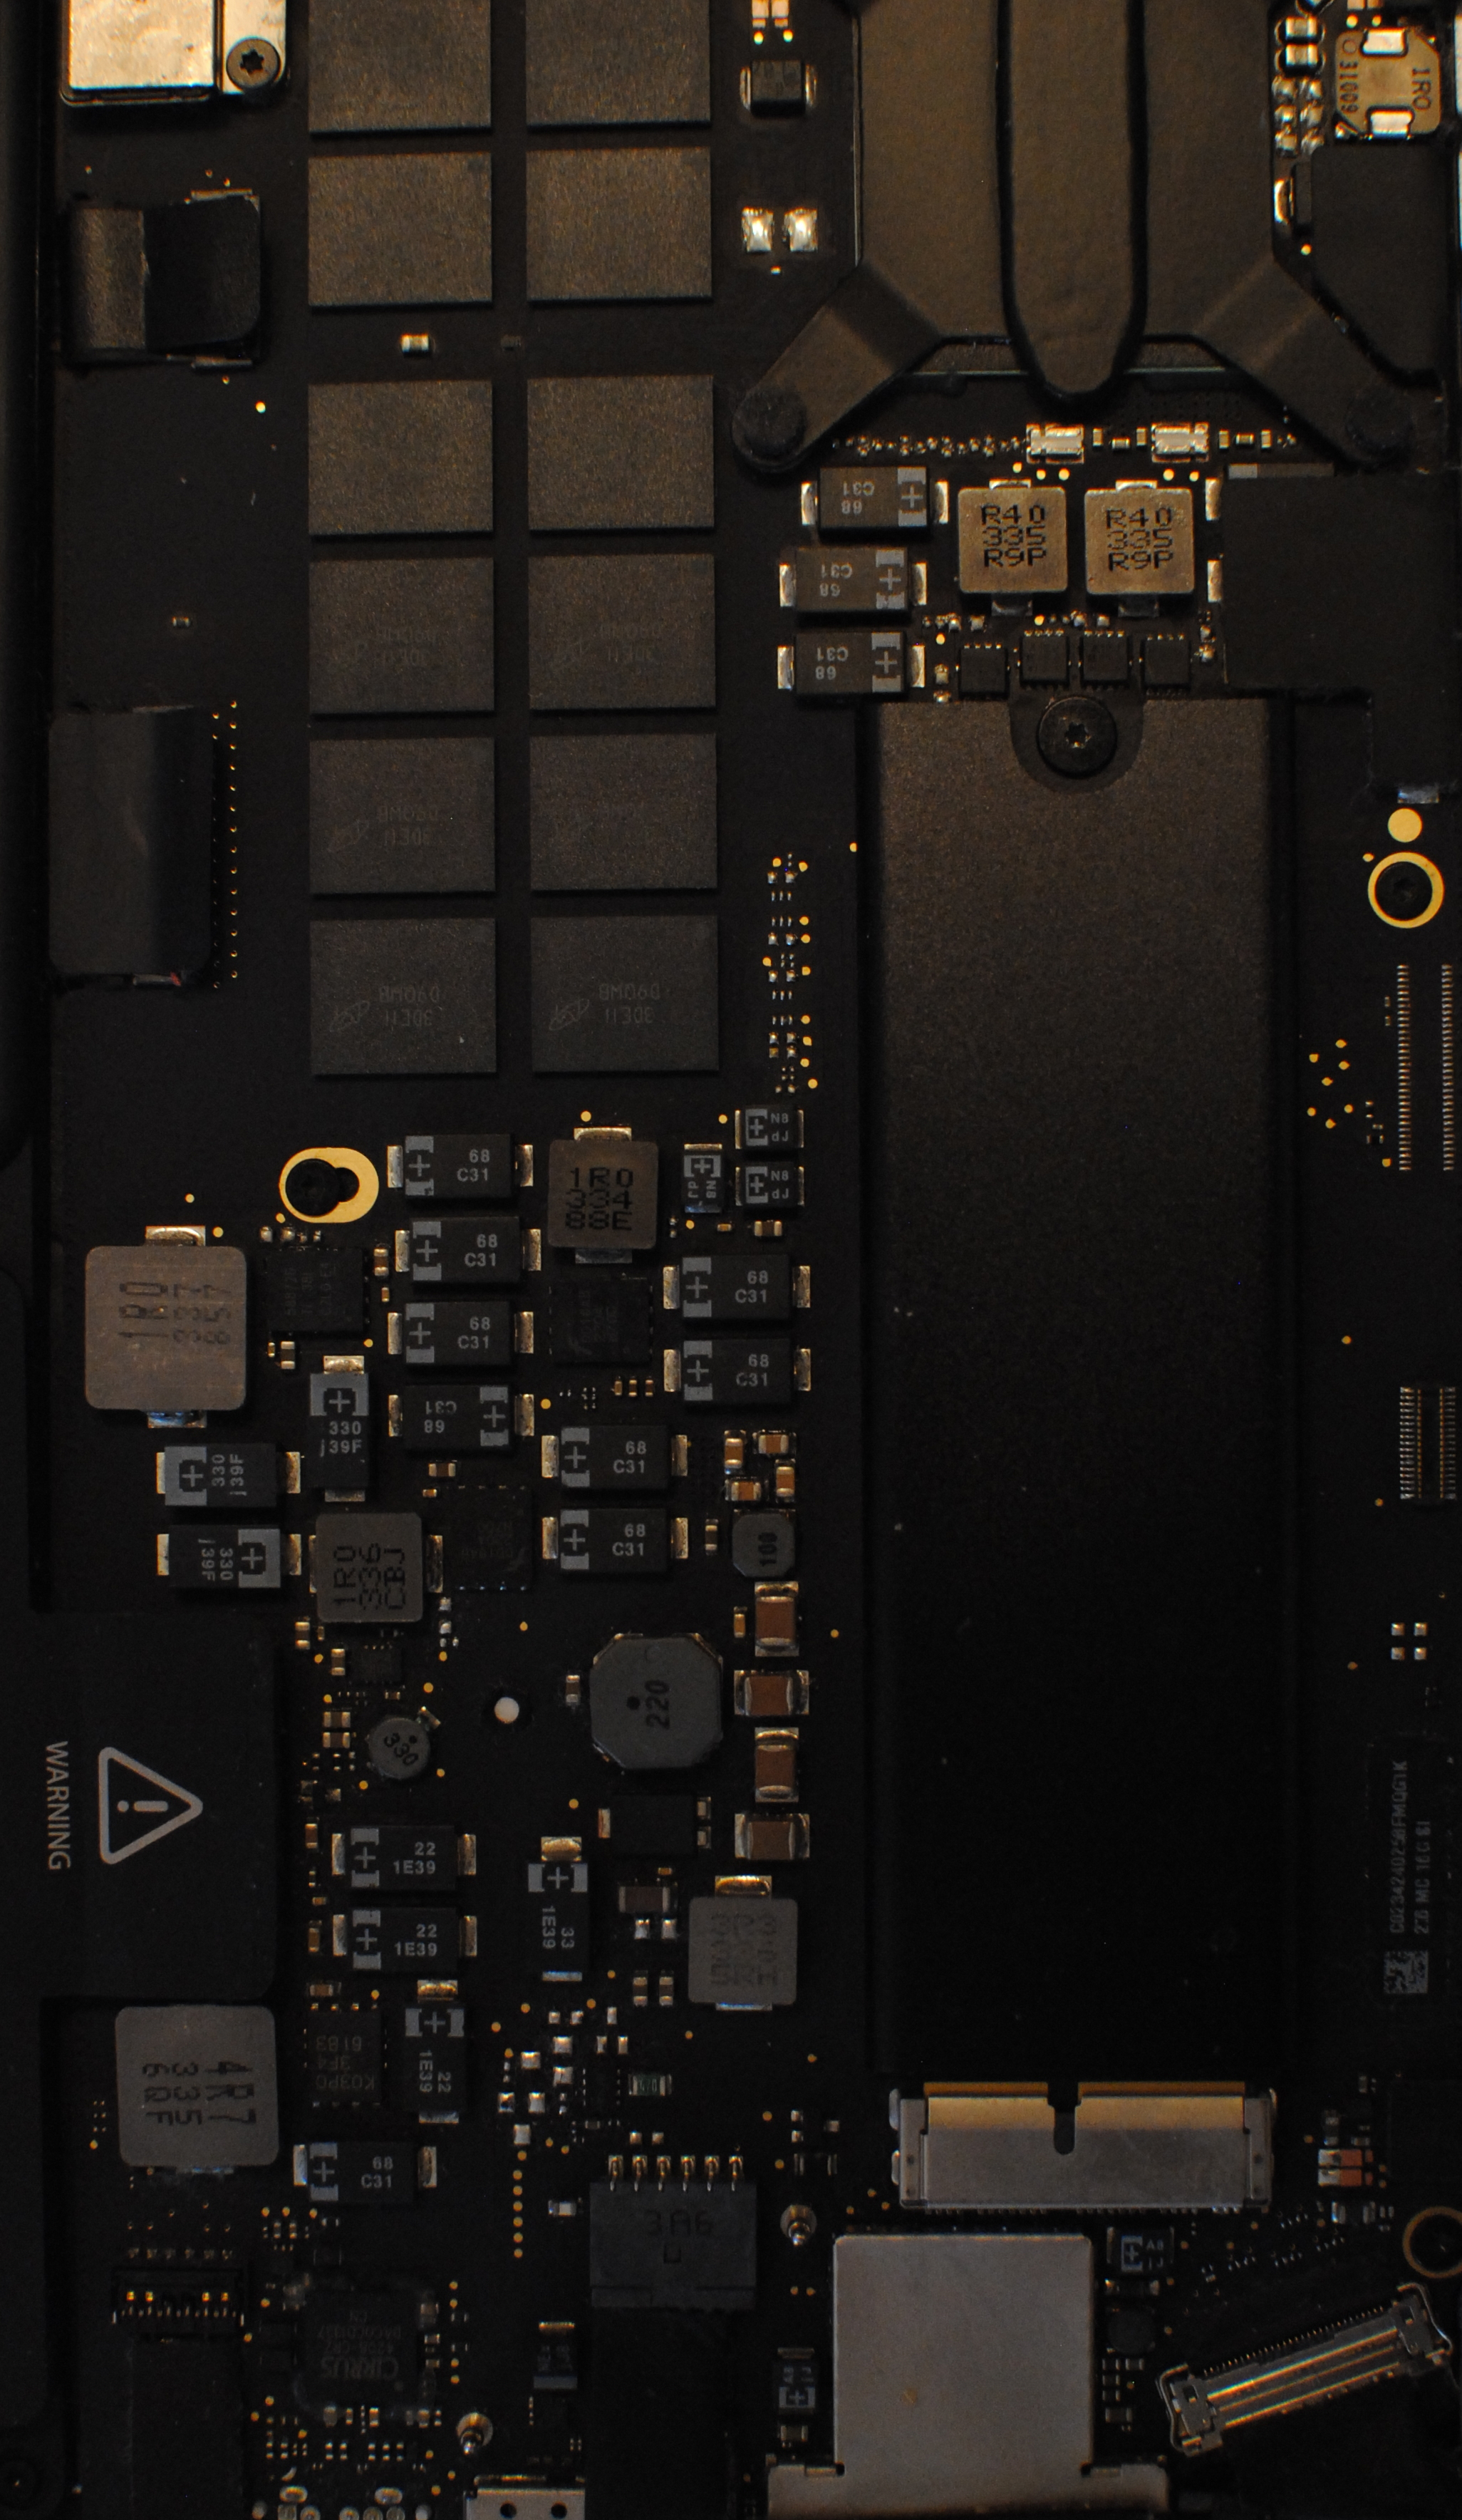
\includegraphics[scale=0.2]{figures/experiments/img.JPG}}

    \subfloat[Some cool related graphic]
    {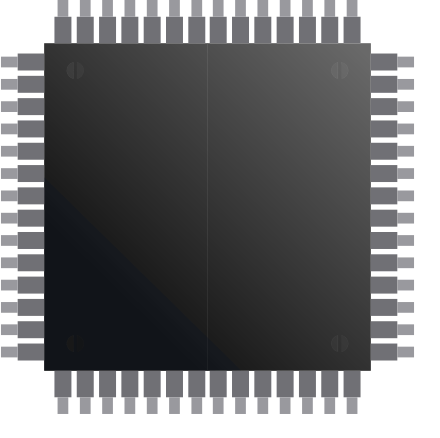
\includegraphics[scale=0.4]{figures/experiments/microcontroller.png}}
    \caption[Caption that appears in the figlist]{\textbf{Caption that appears under the fig} This plot shows...}
    \label{fig:pcaclasses}
\end{centering}
\end{figure}
\begin{table}[ht]
\begin{center}
    \begin{tabular}{|l|r|}
        \hline
        Type & Accuracy\\ \hline
        A    & 82.47 $\pm$ 3.21 \\
        B    & 78.47 $\pm$ 2.43 \\
        C    & 84.30 $\pm$ 2.35 \\
        D    & 86.81 $\pm$ 3.01 \\
        \hline
    \end{tabular}
    \end{center}

    \caption[Table caption]{\textbf{Table caption.} foo bar...\\}
    \label{tab:accuracy}
\end{table}
    \chapter{Related Work}\label{chap:relatedwork}
Give a brief overview of the work relevant for your thesis.
Closely related work should be compared in depth: what are the pros and cons of their work compared to yours?

    \chapter{Conclusion}\label{chap:conclusion}

Brief wrapup of the achievements of this thesis.

Directions for future work (if applicable).


    % bibliography is not in the table of contents per default, add it manually
    % enable the \renewcommand for german header
    % \renewcommand{\bibname}{Literaturverzeichnis}
    \addcontentsline{toc}{chapter}{Bibliography}

    \bibliographystyle{plainnat}
    \bibliography{bib/topic1,bib/topic2}
    \newpage
    \thispagestyle{empty}
    \mbox{}


\end{document}
